\paragraph{Example 1}{
\begin{lstlisting}[language=Python]
from BNumMet.Random import lehmers_rand
for i in range(10):
    print(lehmers_rand())

>> Lehmers Random Number Generator Initialized with default values
	a=16807
	c=0
	m=2147483647
	x=1.0
    7.826369259425611e-06
    0.13153778814316625
    0.7556053221950332
    0.4586501319234493
    0.5327672374121692
    0.21895918632809036
    0.04704461621448613
    0.678864716868319
    0.6792964058366122
    0.9346928959408276
\end{lstlisting}
}
\paragraph{Example 2}{
\begin{lstlisting}[language=Python]
from BNumMet.Random import lehmers_rand, clear_lehmers_vars
clear_lehmers_vars()
arr = [1]
for i in range(10):
    aux = lehmers_rand(a=2**16 + 3, m=2**31, c=0, x=arr[-1])
    if len(arr) >= 3:
        lehmerFormula = (6 * arr[-1] - 9 * arr[-2]) % 1  # Test Xn = (6Xn-1 - 9Xn-2)
        print(f"Lehmer's = {aux}\nPredicted = {lehmerFormula}\n")
    arr.append(aux)

>>  Lehmer's = 0.0008239871822297573
    Predicted = 0.0008239871822297573
    
    Lehmer's = 0.003295936156064272
    Predicted = 0.003295936156064272
    
    Lehmer's = 0.012359732296317816
    Predicted = 0.012359732296317816
    
    Lehmer's = 0.04449496837332845
    Predicted = 0.04449496837332845
    
    Lehmer's = 0.15573221957311034
    Predicted = 0.15573221957311034
    
    Lehmer's = 0.533938602078706
    Predicted = 0.533938602078706
    
    Lehmer's = 0.8020416363142431
    Predicted = 0.8020416363142431
    
    Lehmer's = 0.006802399177104235
    Predicted = 0.006802399177104235
\end{lstlisting}
}
\paragraph{Example 3}{
\begin{lstlisting}[language=Python]
from BNumMet.Random import lehmers_rand, clear_lehmers_vars
clear_lehmers_vars()
fail2 = (
    lambda: float(
        (int(lehmers_rand(a=65539, c=0, m=2**31, x=123) * (2**31)) >> 23) & 0xFF
    )
    / 255
)
fail = [(fail2(), fail2()) for i in range(100000)]
plt.scatter(*zip(*fail), s=1, c="black")
plt.show()
\end{lstlisting}
\begin{figure}[H]
    \centering
    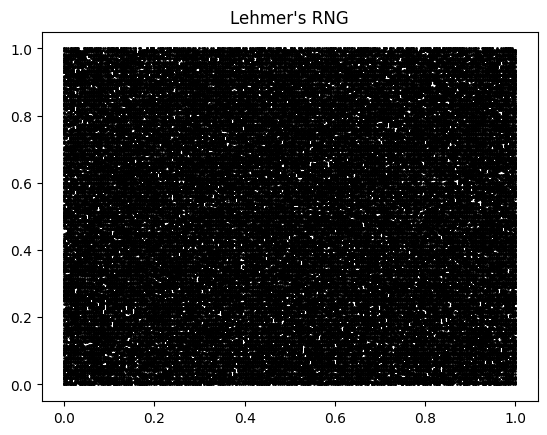
\includegraphics{Include/Images/Thesis/Documentation/Randomness/Lehmers Rand Example 3.png}
    \caption{Lehmers Rand Example 3}
    \label{fig:Lehmers Rand Example 3}
\end{figure}
}
